%% ============================================================================
%% §1 Introduction  --  joint
%% ============================================================================
\section{Introduction}
\label{sec:intro}

\paragraph{Goal.} This project builds an INT8 hybrid CNN accelerator that runs the full 50-layer MobileFaceNet inference flow on-device, producing a 128-dimensional face embedding with no host intervention between layers. The accelerator targets edge use cases (mobile face unlock, on-device door access, in-camera identification) where the operating envelope is sub-100\,mW at real-time frame rates.

\paragraph{Approach overview.} Rather than building a fully programmable NPU, we specialise the datapath around MobileFaceNet's actual operator mix. The accelerator contains three operator engines behind a shared Switcher: a 14$\times$16 systolic array for $1\times1$ convolutions (which account for $\sim$92\,\% of the network's compute), a $3\times3$ standard array for $3\times3$ standard and depthwise convolutions, and a dedicated $7\times7$ depthwise engine for the global pooling layer. All weights, activations, and outputs are INT8, with the model trained via the QuantFace flow~\cite{9955645}.

The same RTL is brought up along two implementation tracks. The Zynq UltraScale+ FPGA bitstream provides hardware-in-the-loop verification of the full PS-PL data path; the FreePDK45 Innovus flow provides ASIC-level area, power, and timing data with full-flow signoff (Genus synthesis, Innovus place-and-route, SDF-annotated gate-level simulation). Both tracks execute the same 19.18\,M cycles per inference and have been verified bit-exact against the same C-model golden reference.

\paragraph{Prior art.} The MobileFaceNet topology is from Chen et al.~\cite{chen2018mobilefacenetsefficientcnnsaccurate}, with the non-square $112\times96$ input variant from Sun et al.~\cite{Linjun_SUN20202019EDL8103}. The INT8 quantisation flow and the face-verification benchmark suite (LFW, CFP, AgeDB, CALFW, CPLFW, IJB-B/C) follow QuantFace~\cite{9955645}. The systolic-array dataflow draws on Eyeriss~\cite{7738524}; the closely related edge-deployment model EdgeFace~\cite{george2024edgefaceefficientfacerecognition} targets the same use case at the model level, whereas our contribution is the hardware track.

\begin{figure}[H]
  \centering
  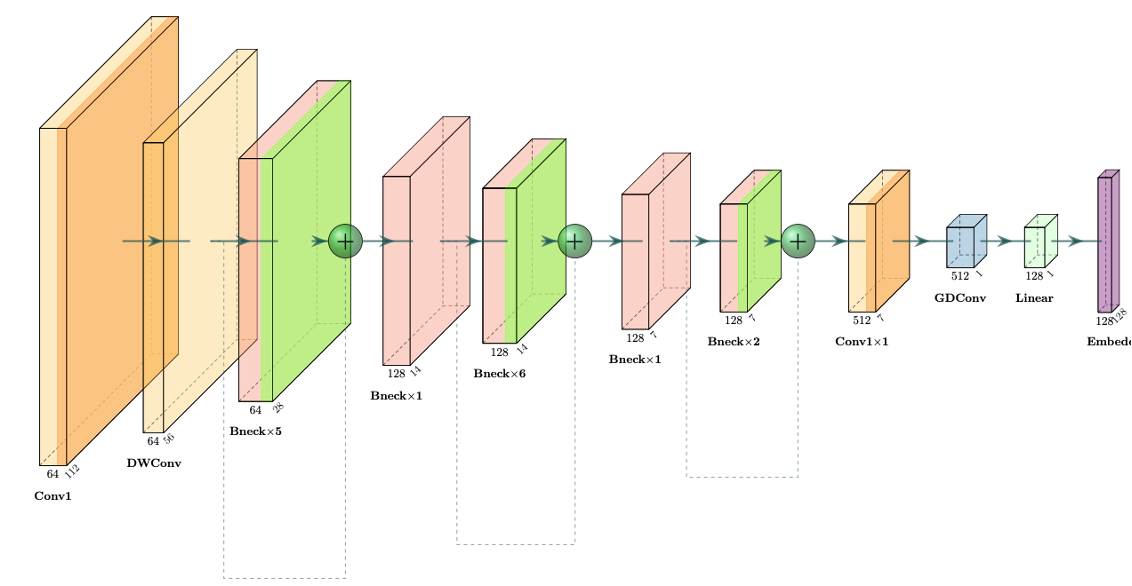
\includegraphics[width=0.95\textwidth]{Fig/old/mobile_face_net_visualize.png}
  \caption[MobileFaceNet topology overview.]{MobileFaceNet topology overview: 50 layers from the initial $3\times3$ convolution through five bottleneck stages to the final $7\times6$ global depthwise convolution and $1\times1$ linear projection producing a 128-d embedding.}
  \label{fig:mobilefacenet}
\end{figure}

\paragraph{Report structure.} Section~\ref{sec:model} fixes the model topology and INT8 quantisation. Section~\ref{sec:broader} discusses broader impacts and Section~\ref{sec:constraints} states design constraints. Section~\ref{sec:hw} describes the hardware architecture (shared frontend and the two backend tracks). Section~\ref{sec:opt} walks through the architectural optimisation journey. Section~\ref{sec:standards} lists engineering standards. Section~\ref{sec:verify} presents functional and timing verification. Section~\ref{sec:ethics} addresses ethical considerations specific to face recognition. Section~\ref{sec:conclusion} concludes.
